\let\negmedspace\undefined
\let\negthickspace\undefined
\documentclass[journal,12pt,twocolumn]{IEEEtran}
\usepackage{cite}
\usepackage{amsmath,amssymb,amsfonts,amsthm}
\usepackage{algorithmic}
\usepackage{graphicx}
\usepackage{textcomp}
\usepackage{xcolor}
\usepackage{txfonts}
\usepackage{listings}
\usepackage{enumitem}
\usepackage{mathtools}
\usepackage{gensymb}
\usepackage{comment}
\usepackage[breaklinks=true]{hyperref}
\usepackage{tkz-euclide} 
\usepackage{listings}
\usepackage{gvv}                                        
\def\inputGnumericTable{}                                 
\usepackage[latin1]{inputenc}                                
\usepackage{color}                                            
\usepackage{array}                                            
\usepackage{longtable}                                       
\usepackage{calc}                                             
\usepackage{multirow}                                         
\usepackage{hhline}                                           
\usepackage{ifthen}                                           
\usepackage{lscape}

\newtheorem{theorem}{Theorem}[section]
\newtheorem{problem}{Problem}
\newtheorem{proposition}{Proposition}[section]
\newtheorem{lemma}{Lemma}[section]
\newtheorem{corollary}[theorem]{Corollary}
\newtheorem{example}{Example}[section]
\newtheorem{definition}[problem]{Definition}
\newcommand{\BEQA}{\begin{eqnarray}}
\newcommand{\EEQA}{\end{eqnarray}}
\newcommand{\define}{\stackrel{\triangle}{=}}
\theoremstyle{remark}
\newtheorem{rem}{Remark}
\begin{document}
\bibliographystyle{IEEEtran}
\vspace{3cm}
\title{GATE 2022 ME-32}
\author{EE23BTECH11027 - K RAHUL$^{*}$% <-this % stops a space
}
\maketitle
\newpage
\bigskip
\renewcommand{\thefigure}{\theenumi}
\renewcommand{\thetable}{\theenumi}
\textbf{Question:}\\
A rigid uniform annular disc is pivoted on a knife edge A in a uniform gravitational
field as shown, such that it can execute small amplitude simple harmonic motion in
the plane of the figure without slip at the pivot point. The inner radius $r$ and outer
radius $R$ are such that $r^2 = \frac{R^2}{2}$, and the acceleration due to gravity is $g$. If the
time period of small amplitude simple harmonic motion is given by $T = \beta \pi \sqrt{\frac{R}{g}}$,
where $\pi$ is the ratio of circumference to diameter of a circle, then $\beta$ =  (Round off to 2 decimal places)
\begin{figure}[h]
    %\caption{Stem Plot of $x(n)$ v/s n}
    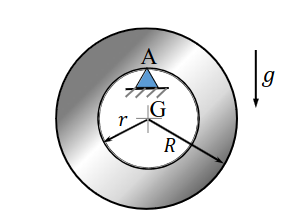
\includegraphics[width=0.4\textwidth]{figs/11027_GATE_ME_32.png}\label{11027_GATE_ME_32}
    \caption{Question Diagram}
\end{figure}
\hfill{GATE 2022 ME-32}
\\
\bigskip \bigskip


\solution
\begin{table}[ht]
\setlength{\arrayrulewidth}{0.3mm}
\setlength{\tabcolsep}{15pt}
\renewcommand{\arraystretch}{1.5}

table 1\\

\begin{tabular}{ |p{1cm}|p{3cm}|p{1cm}| }
\hline
\multicolumn{3}{|c|}{Parameters in expression}\\
\hline
Symbol & Description & Value\\
\hline
n & The nth term of series & To be computed\\
\hline
$a_n$ & nth term of series & 350\\
\hline
$a_0$ & 0th term of series & 17 \\
\hline
d & Common difference of AP & 9\\
\hline
\end{tabular}


\end{table}


Moment of inertia of disc about pivot point is calculated as
\begin{align}
	I &= \frac{1}{2}\brak{R^2 + \frac{R^2}{2}} + \frac{MR^2}{2} \\
	&= \frac{5}{4}MR^2 \label{11027_Moment_Of_Inertia}
\end{align}

Using D' Alambert's principle,
\begin{align}
	&I\frac{d^2\theta \brak{t}}{dt^2} + mgr\sin\brak{\theta \brak{t}} = 0\\
	\implies& I\frac{d^2\theta \brak{t}}{dt^2} + mgr\theta \brak{t}= 0,\text{for } \theta \ll 1, \theta > 0 \label{11027_dAlambert_principle}
\end{align}

Using \eqref{11027_Moment_Of_Inertia} and \eqref{11027_dAlambert_principle}, we get
\begin{align}
	\frac{5MR^2}{4}&\frac{d^2 \theta \brak{t}}{dt^2} + Mg\frac{R}{\sqrt{2}} \theta \brak{t} = 0\\
	&\frac{d^2 \theta \brak{t}}{dt^2} + \frac{2\sqrt{2}g}{5R} \theta \brak{t}= 0 	
\end{align}
\\
Taking Laplace Transform on both sides,we get
\begin{align}
	s^2\alpha \brak{s} &- s \theta \brak{0} - \theta ' \brak{0} + \frac{2\sqrt{2}g}{5R} \alpha\brak{s}= 0\\
	\alpha\brak{s}&\brak{s^2+\frac{2\sqrt{2}g}{5R}} = \theta ' \brak{0}\\
	\alpha\brak{s}&= \frac{\theta ' \brak{0}}{\brak{s^2 + \frac{2\sqrt{2}g}{5R}}} \label{11027_alpha_s}
\end{align}
\\
\begin{align}
	u\brak{t}&\system{L}\frac{1}{s}\\
	e^{at}u\brak{t}&\system{L}\frac{1}{s-a}\\
	\frac{\brak{e^{jat} - e^{-jat}}}{2}u\brak{t}&\system \frac{a}{s^2+a^2}\\
	\sin\brak{at}&\system\frac{a}{s^2+a^2} \label{11027_Laplace_of_sine}
\end{align}
From \eqref{11027_alpha_s} and \eqref{11027_Laplace_of_sine}
\begin{align}
	\alpha\brak{s}&= \frac{\theta ' \brak{0} \brak{\sqrt{\frac{2\sqrt{2}g}{5R} }} }{\brak{s^2 + \frac{2\sqrt{2}g}{5R}}} \frac{1}{ \brak{\sqrt{\frac{2\sqrt{2}g}{5R} }} }
\end{align}
\\
Taking inverse Laplace by putting $\frac{\theta ' \brak{0}}{\brak{\sqrt{\frac{2\sqrt{2}g}{5R}}}} = k$ and \eqref{11027_Laplace_of_sine}, 
\begin{align}
	\theta \brak{t} &= k \sin\brak{\frac{2\sqrt{2}g}{5R} t}\\
	T &= \frac{2 \pi}{\frac{2\sqrt{2}g}{5R}}\\
	&= \sqrt{\brak{5\sqrt{2}}}\:\pi \sqrt{\frac{R}{g}}
\end{align}
Thus, 
\begin{align}
	\beta = \sqrt{\brak{5\sqrt{2}}}\\
	\beta = 2.66
\end{align}
\end{document}
